%---------- Inleiding ---------------------------------------------------------

\section{Introductie}\sloppy
\label{sec:introductie}

Het gebruik van een online agenda wordt alsmaar populairder. Er zijn hiervoor veel gekende oplossingen zoals Google Agenda, maar in het project van het bedrijf TurnUp, wordt er een eigen kalendertoepassing ontwikkeld. Hierdoor wordt het onoverzichtelijk voor de gebruiker, wanneer er meerdere kalenders door elkaar gebruikt worden. Een oplossing hiervoor is om de verschillende kalenders met elkaar te synchroniseren. Google Agenda kan gesynchroniseerd worden met andere kalenders zoals Microsoft Outlook. Maar om met een zelfontwikkelde kalender te synchroniseren, zou een grote verandering nodig zijn van de huidige software van TurnUp.

Het doel van deze studie is dus om te onderzoeken hoe het bedrijf, TurnUp, de eigen kalenderimplementatie kan synchroniseren met Google Agenda, en wat de technische en praktische overwegingen zijn die daarbij komen kijken.

%---------- Stand van zaken ---------------------------------------------------

\section{State-of-the-art}%
\label{sec:state-of-the-art}

In deze studie wordt onderzocht hoe het bedrijf, TurnUp, haar eigen kalenderimplementatie kan synchroniseren met Google Agenda, en wat de technische en praktische overwegingen zijn die daarbij komen kijken.

Het synchroniseren van een agenda is heel belangrijk voor de samenwerking in een omgeving. Zo kan een team gemakkelijk de projectactiviteiten opvolgen op deze manier \autocite{Xhafa2016}.

Een probleem met synchronisatie is dat alle verbonden apparaten zo snel mogelijk de laatste aanpassingen moeten hebben. Dit is voor sommige apparaten moeilijk wanneer ze tijdelijk geen internetconnectie hebben. 
Daarom moet er een manier zijn om te gebruiker toch te laten weten dat er veranderingen zijn gebeurd in de kalender \autocite{Xhafa2016}.
 
Een ander probleem uit de paper van \textcite{Xhafa2016} is de conflicten die zich kunnen voordoen wanneer meerdere gebruikers een bepaalde activiteit in de agenda aanpassen.
Met Google Agenda is dit geen probleem, aangezien er automatisch aan ``Conflict report'' wordt gedaan \autocite{Google2023}.
Het conflict zal gerapporteerd worden aan de gebruikers zodat dit kan opgelost worden. 

Het bedrijf, TurnUp, wil de agendasynchronisatie uitwerken aan de hand van Google Agenda. Dit is natuurlijk een van de meer populaire software oplossingen voor agendasynchronisatie.
In de masterthesis van \textcite{Vladimir2016}, is er onderzocht hoe een ander bedrijf kan overstappen van een Microsoft Exchange server, naar een Google variant. 
Dit bedrijf wou overstappen omdat het gebruik van Microsoft Exchange server, hen niet toeliet om andere e-mailproviders te gebruiken. Deze versie van de agenda liet hun ook enkel toe om eenvoudige evenementen aan te maken in de agenda. 

Voor de integratie van Google Agenda zijn er verschillende vereisten. 
Er is een OAuth-scherm nodig, een Google Cloud project, een Google account en de Google Calendar API \autocite{Google2023a}.
Hoe de integratie exact uitgevoerd moet worden, zal afhankelijk zijn in welke programmeertaal deze moet geïmplementeerd worden. 

%---------- Methodologie ------------------------------------------------------
\section{Methodologie}%
\label{sec:methodologie}
\subsection{Fase 1: Literatuurstudie}
De doelstelling in de eerste fase is het onderzoeken van het kalendersysteem bij TurnUp. Tijdens dit onderzoek zullen ook relevante hulpmiddelen geïdentificeerd worden, die gebruikt kunnen worden in het verdere verloop van het onderzoek. Ook zal er in deze fase gezocht worden naar relevante bronnen en bestaande onderzoeken met betrekking tot het onderwerp.
Deze fase zal ongeveer twee weken duren. 

\subsection{Fase 2: Casusbeschrijving (AS IS)}
In de tweede fase zal er een uitgebreide beschrijving gemaakt worden van hoe het kalendersysteem nu gebruikt wordt door klanten van TurnUp. Dit zal gebeuren aan de hand van een of meerdere interviews. Hieruit zal er meer duidelijkheid komen over waarom een gedeelde Google Agenda beter en efficiënter is. 
Deze fase zal ongeveer twee weken duren.

\subsection{Fase 3: Requirement-analyse (TO BE)}
In deze fase zal er onderzocht worden wat er nodig is om de synchronisatie met Google Agenda efficiënt te integreren. Dit is aan de software kant bij TurnUp maar ook aan de kant van de klanten van TurnUp.
Aan het eind van deze fase zal een lijst met vereisten gemaakt zijn.
Deze fase zal ongeveer een week duren. 

\subsection{Fase 4: Shortlist van hulpmiddelen}
In fase vier zal er een lijst van hulpmiddelen opgemaakt worden. Dit zal gedaan worden door de hulpmiddelen van de eerste fase te evalueren. Deze hulpmiddelen kunnen gebruikt worden voor het efficiënt te synchroniseren van de Google Agenda en de eigen kalenderimplementatie.
Dit zal gedaan worden door met medewerkers van TurnUp in gesprek te gaan. Zij kunnen hun ervaringen en mogelijke hulpmiddelen delen. Uit de opgemaakte lijst kan beslist worden welke hulpmiddelen het best zijn om te gebruiken tijdens de integratie.
Deze fase zal ongeveer een week duren. 

\subsection{Fase 5: Integratie} 
Tijdens deze fase zal, aan de hand van de eerder geselecteerde hulpmiddelen, de integratie plaatsvinden. 
Het doel van deze fase is een werkende integratie te realiseren om uit te testen en te analyseren.
Deze fase zal ongeveer vier weken duren. 

\subsection{Fase 6: Analyse en evaluatie}
In deze fase zal de integratie uit de vorige fase geanalyseerd worden. Dit met behulp van de werknemers bij TurnUp.
Uit deze fase kan er een analyseverslag gemaakt worden waaruit de uiteindelijke conclusies getrokken kunnen worden.
Deze fase zal ongeveer twee weken duren


\subsection{Fase 7: Rapportering en documentatie}
In fase zeven zal het hele onderzoek en de conclusies hiervan gedocumenteerd worden.
Dit zal gebeuren aan de hand van alle verzamelde informatie doorheen het semester. 
Aan het einde van deze fase zal de bachelorproef voltooid zijn. 
Deze fase zal ongeveer een week duren.

\subsection{Fase 8: Review en afronding}
Tijdens deze fase zal alles nog eens grondig herbekeken worden. 
De documentatie wordt gecheckt op fouten en wordt klaargemaakt om in te dienen. 
Aan het einde van deze fase zal de bachelorproef klaar zijn om ingediend te worden en is het onderzoek afgelopen.
Deze fase zal ongeveer een week duren. 
\begin{figure}
    \centering
    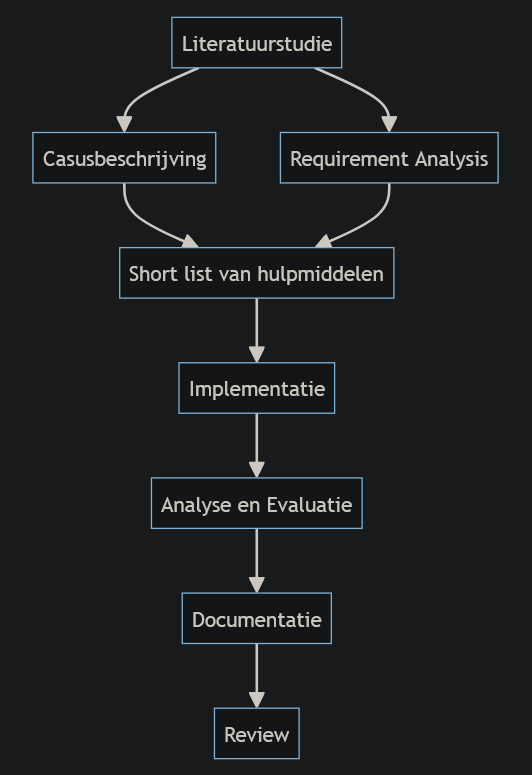
\includegraphics[width=0.7\linewidth]{graphics/flowchart}
    \caption{flowchart}
    \label{fig:flowchart}
\end{figure}

%---------- Verwachte resultaten ----------------------------------------------
\section{Verwacht resultaat, conclusie}%
\label{sec:verwachte_resultaten}
Dit onderzoek moet leiden tot een efficiënter en eenvoudiger gebruik van de software van TurnUp. De klanten zullen Google Agenda kunnen gebruiken om een gecentraliseerde agenda te hebben. 
Ze zullen geen nood meer hebben aan verschillende agenda's.
Dit zal de software van TurnUp ook een boost geven aangezien de efficiëntie van hun product stijgt dankzij dit onderzoek. 

